%\begin{frame}
%\frametitle{Neutrinos through the looking glass}
%
%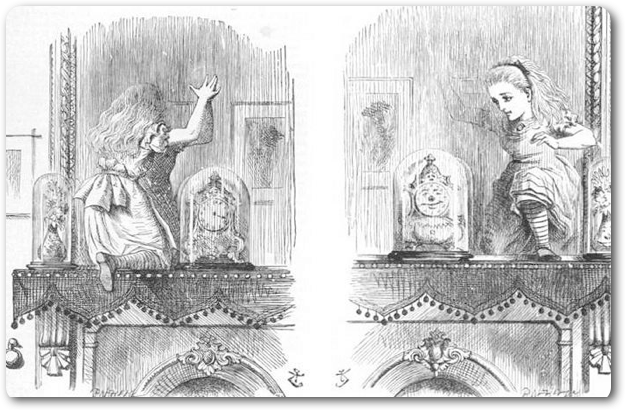
\includegraphics[scale=0.4]{img/Alice.png}
%
%\end{frame}


%\begin{frame}
%\frametitle{Parity}
%\begin{columns}
%\column{0.5\textwidth}
%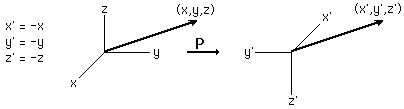
\includegraphics[scale=0.45]{img/ParityCartoon.png}
%
%
%The parity transformation changes a right-handed coordinate system into a left-handed one or vice versa. Two applications of the parity transformation restores the coordinate system to its original state.
%
%It is a reasonable presupposition that nature should not care whether its coordinate system is right-handed or left-handed, \alert{but surprisingly, that turns out not to be so.}
%
%\column{0.5\textwidth}
%%\begin{block}{}
%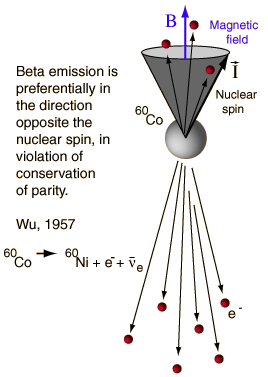
\includegraphics[scale=0.35]{img/wu.png}
%
%In 1956, T. D. Lee and C. N. Yang predicted the non conservation of parity in the weak interaction. Their prediction was quickly tested when C. S. Wu and collaborators studied the beta decay of Cobalt-60 in 1957.
%
%%\end{block}
%\end{columns}
%
%\end{frame}

%\begin{frame}
%\includegraphics[scale=0.35]{Cobalt.png}
%%wu.png
%\end{frame}
%GoldhaberExperiment.png
%\begin{frame}
%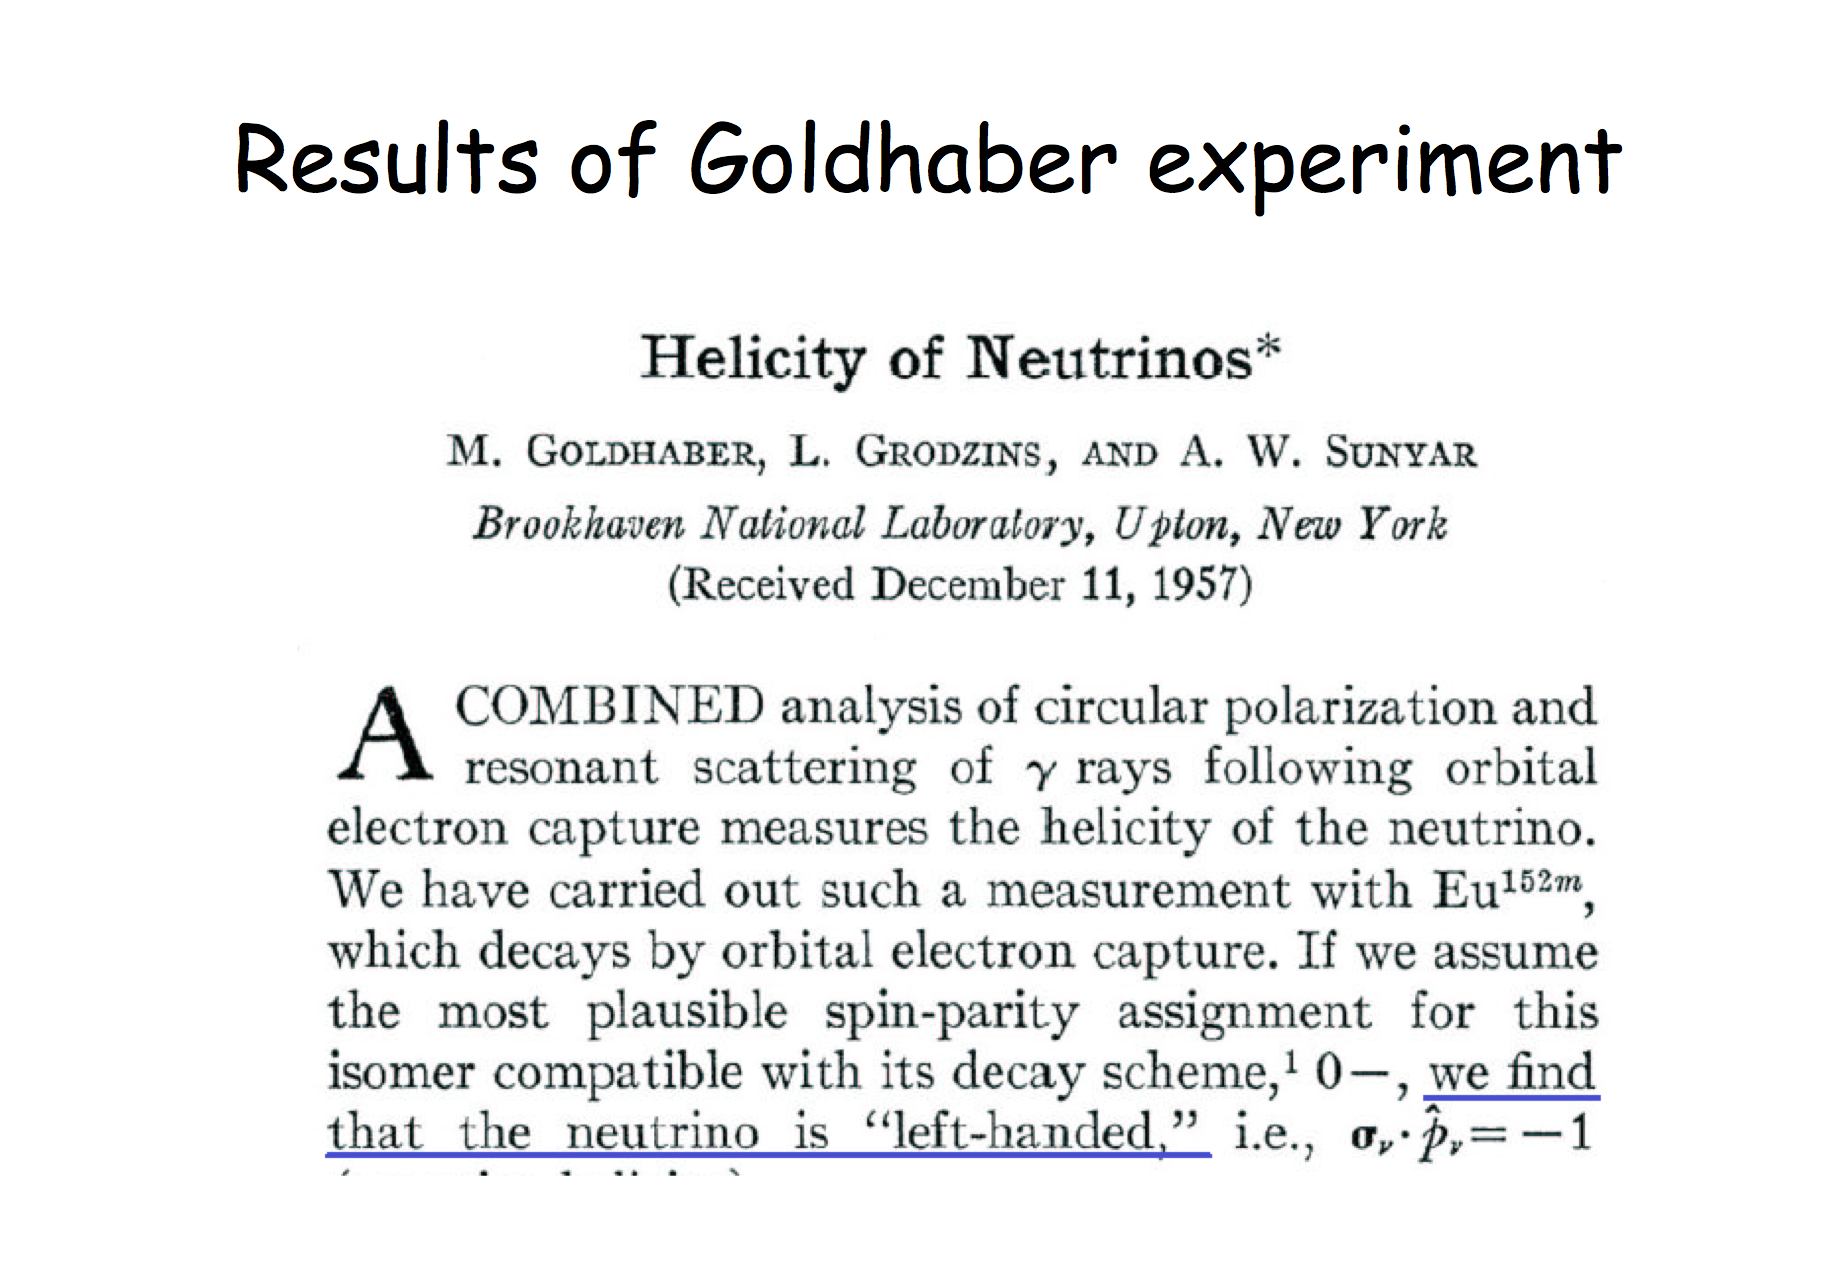
\includegraphics[scale=0.35]{img/Goldhaber.png}
%
%\end{frame}
%
%\begin{frame}
%\frametitle{What do we talk about when we talk about helicity?}
%\begin{columns}
%\column{0.5\textwidth}
%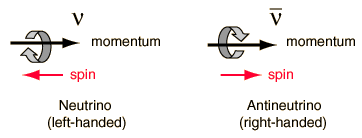
\includegraphics[scale=0.35]{img/NeutrinoHelicity.png}
%
%Helicity is the spin projection in the direction of motion.
%\[
%h = \frac{\va{\sigma}\cdot \va{p}}{p}
%\]
%The Goldhaber experiment measured that neutrinos are left handed (spin opposed to motion, $h=-1$). The CPT theorem ensures that anti-neutrinos must be right-handed (spin along motion, $h=+1$).
%\column{0.5\textwidth}
%
%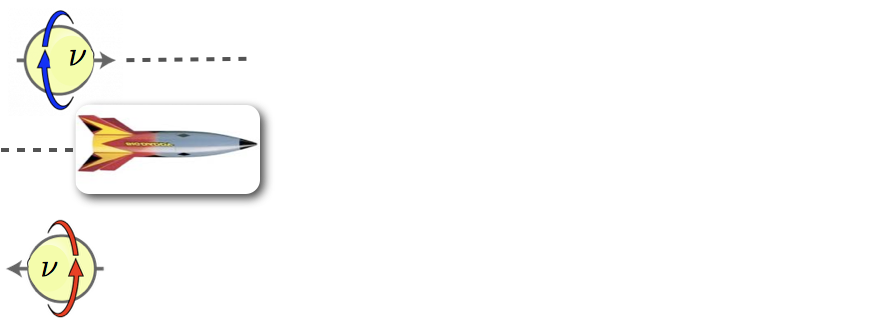
\includegraphics[scale=0.30]{img/neutrinoBoost2.png}
%
%For massive particles, helicity depends on the reference frame and thus is not Lorentz invariant. One can always jump into a reference system faster than that of the particle and see its helicity flip.
%
%But massless particles travel at the speed of light and cannot be overtaken. The helicity becomes a constant of motion. 
%\end{columns}
%
%\end{frame}

%
%\begin{frame}
%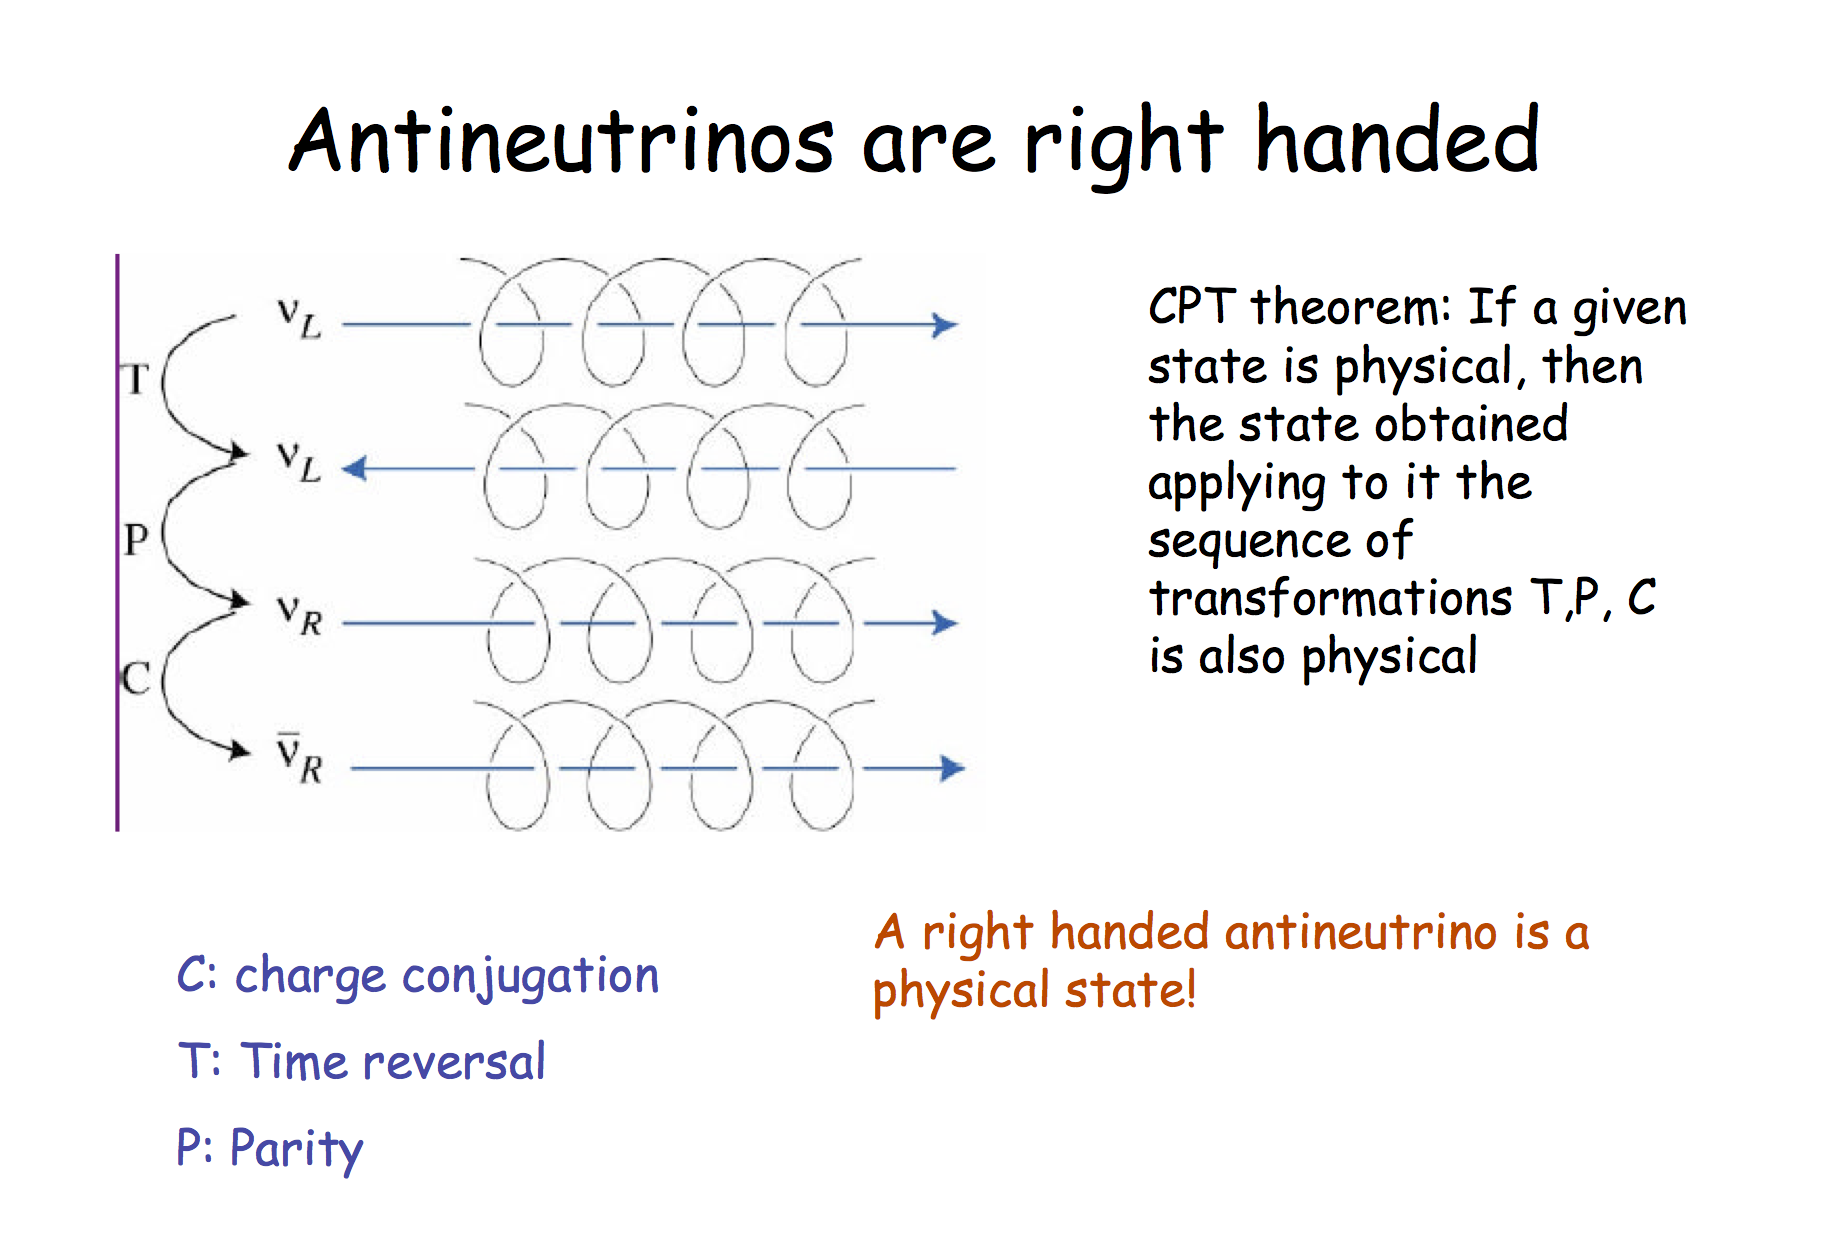
\includegraphics[scale=0.35]{AntineutrinosRH.png}
%
%\end{frame}

\begin{frame}
\frametitle{Massless particles and helicity}
\begin{columns}
\column{0.5\textwidth}
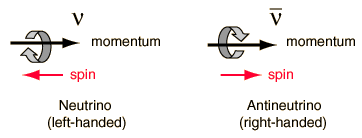
\includegraphics[scale=0.35]{img/NeutrinoHelicity.png}

Helicity is the spin projection in the direction of motion.
\[
h = \frac{\va{\sigma}\cdot \va{p}}{p}
\]
In the limit of $m \rightarrow 0$~ Dirac's equation(s) decouple in 
two states with definite helicity:
 \begin{empheq}[box=\fbox]{align}
(E +  \va{p}\cdot\va{\sigma}) \chi  & = 0 \nonumber \\
(E -  \va{p}\cdot\va{\sigma}) \phi  & = 0 \nonumber
\end{empheq}
The particle has negative helicity and the antiparticle positive helicity. \alert{Massless particles have well defined helicity}.

\column{0.5\textwidth}
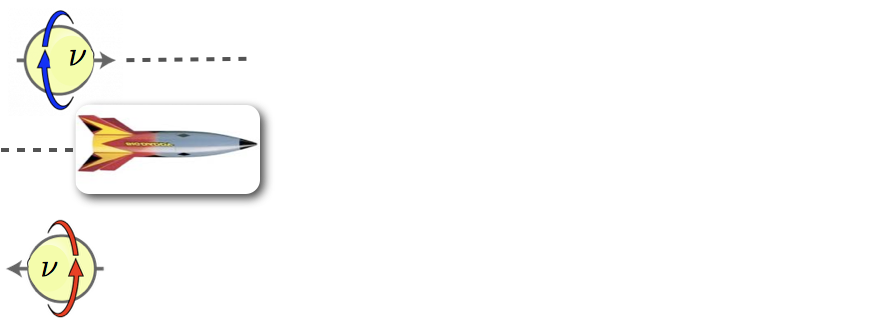
\includegraphics[scale=0.30]{img/neutrinoBoost2.png}

For massive particles, helicity depends on the reference frame. One can always jump into a reference system faster than that of the particle and see its helicity flip.

But massless particles travel at the speed of light and cannot be overtaken. The helicity becomes a constant of motion. 
\end{columns}
\end{frame}

%\begin{frame}
%\frametitle{What do we talk about when we talk about (Standard Model) neutrinos?}
%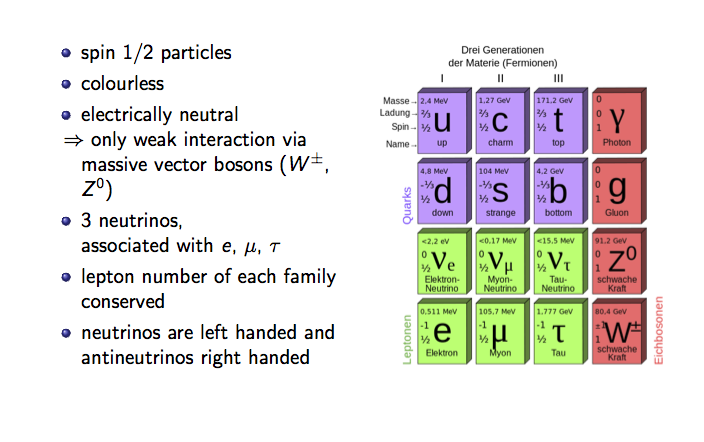
\includegraphics[scale=0.90]{img/NeutrinoOverview.png}
%\end{frame}

\begin{frame}
\frametitle{Neutrinos through the looking glass}
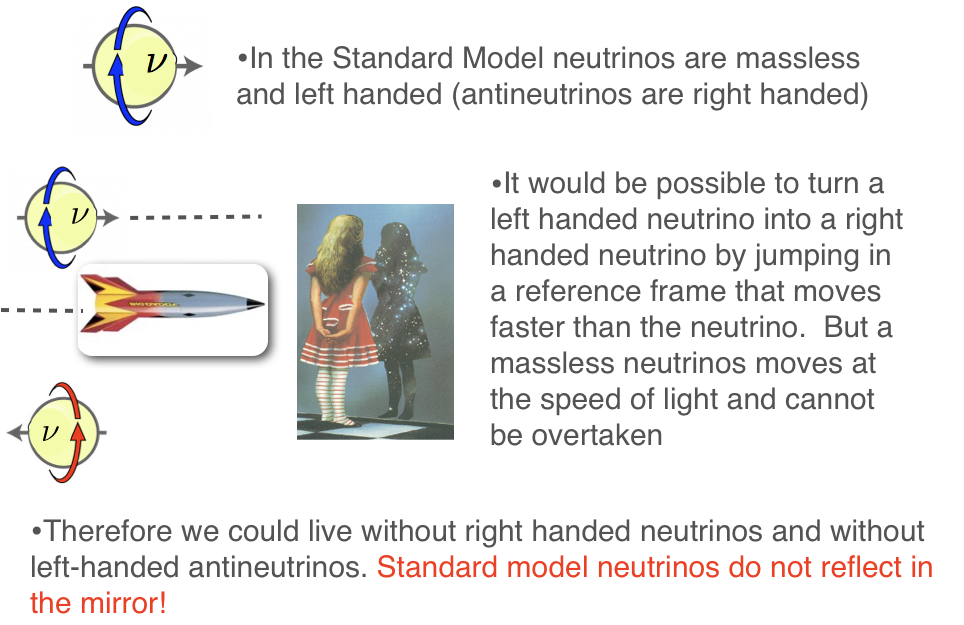
\includegraphics[scale=0.33]{img/NeutrinosLookingG.png}
\end{frame}

\begin{frame}
\frametitle{But what if neutrinos are massive?}
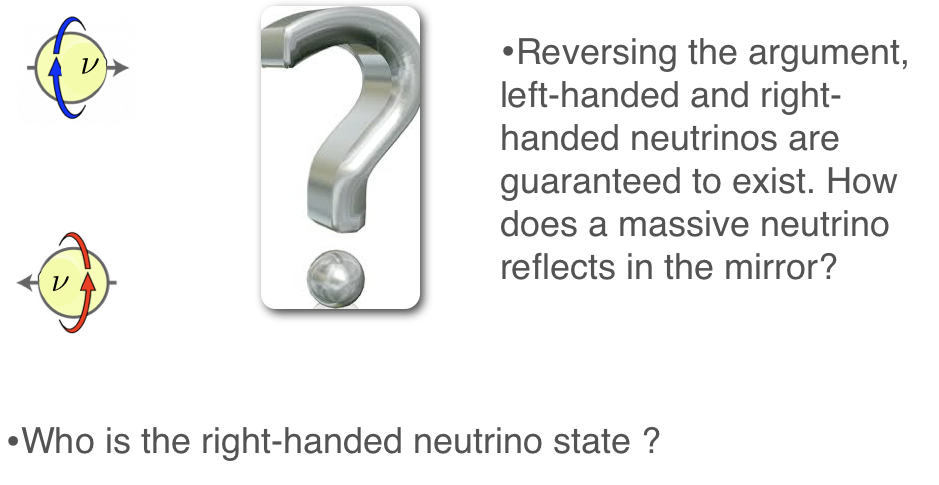
\includegraphics[scale=0.33]{img/WhatIfNeutrinoMassive.png}
\end{frame}

\begin{frame}
\frametitle{Neutrino oscillations}
%\begin{columns}
%\column{0.4\textwidth}
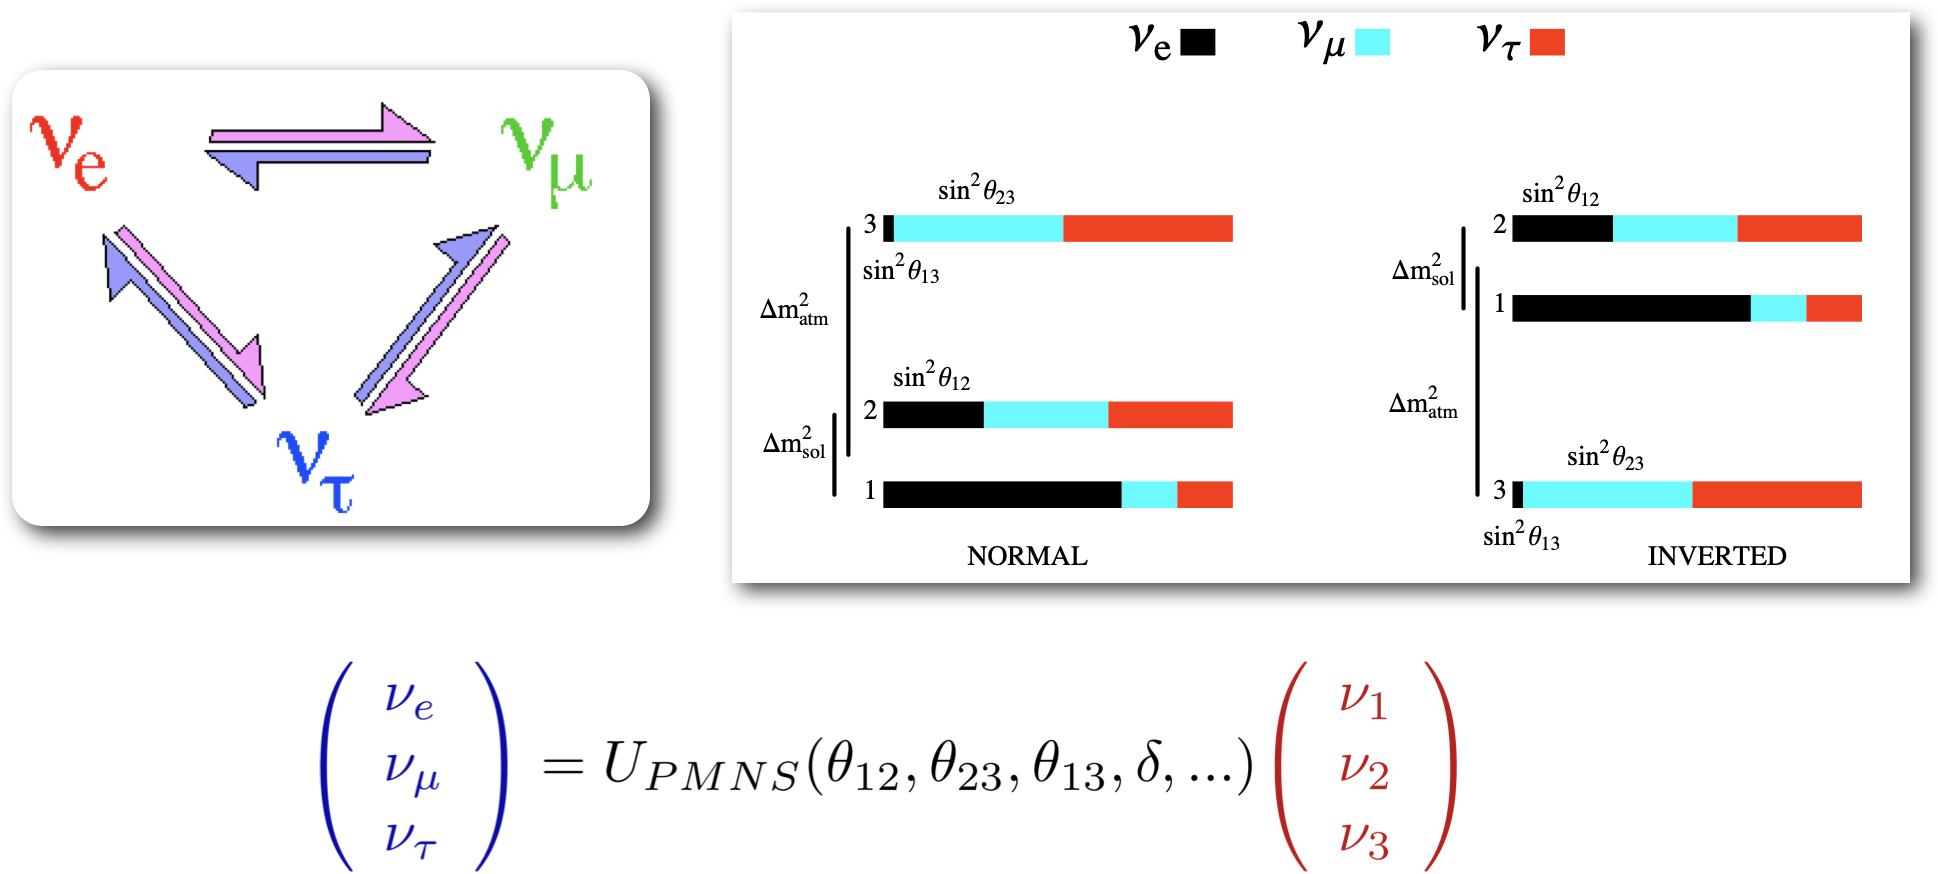
\includegraphics[scale=0.30]{img/neutrinoOscillations.png}
%\column{0.4\textwidth}
%\begin{block}{}

Neutrino oscillation experiments (a story to be told some other time) \alert{have established that neutrinos are massive}. Their mass is, however, very small. Thus, the deviation of the neutrino from a left-handed particle is an effect of order $m/E$~where $m$~is the mass of the neutrino (tiny) and $E$~the energy of the process (usually much larger). 
%\end{block}
%\end{columns}
\end{frame}






